% spedoc.tex V3.0, 13 May 2010

\documentclass[times]{speauth}

\usepackage{moreverb}

\usepackage[colorlinks,bookmarksopen,bookmarksnumbered,citecolor=red,urlcolor=red]{hyperref}

\newcommand\BibTeX{{\rmfamily B\kern-.05em \textsc{i\kern-.025em b}\kern-.08em
T\kern-.1667em\lower.7ex\hbox{E}\kern-.125emX}}

\def\volumeyear{2014}

\begin{document}

\title{Understanding the Modular Operators of \\ Delta-Oriented Programming}

\author{Fausto Carvalho\affil{1},  Marcos Oliveira\affil{1}, Pedro Costa\affil{1}, Alexandre Lucchesi\affil{1}, Rodrigo Bonif\'{a}cio\affil{1}, Hilmer Neri\affil{2}, Daniel Sandoval\affil{1}}

\address{\affilnum{1}Computar Science Department, University of Bras\'{i}lia,
  Bras\'{i}lia, Brazil \break
  \affilnum{2}Faculty of Engineering of Gama, University of Bras\'{i}lia,
  Bras\'{i}lia, Brazil}

\corraddr{Campus Universit\'{a}rio Darcy Ribeiro -- Asa Norte
Edif\'{i}cio CIC/EST 70910-900 Brasília -- DF -- Brasil. Email: rbonifacio@cic.unb.br}

\begin{abstract}
This paper describes the use of the \LaTeXe\
\textsf{\journalclass} class file for setting papers for
\emph{\journalnamelc}.
\end{abstract}

\keywords{Delta Oriented Programming}


\maketitle

\vspace{-6pt}

\section{Introduction}

There is a growing interest in the research and 
development of variant intensive software systems (such as
software product lines~\cite{}), leading to the design of several techniques for
modeling, modularising, implementing,
and reasoning about software variability. That is the case of
Delta-Oriented programming,  a prominent technique for implementing
variant systems that has evolved from an experimental,
prototypical based approach~\cite{schaeger-splc2010}
for dealing with software variability composition 
to a full fledged Java implementation~\cite{koscielny-ppj14}.

In the context of variant intensive software systems,
modularity is recognized as a fundamental property, and the
relation between modularity and variant systems (in general)
is clearly discussed within the Baldwin and Clark theory~\cite{dr-book}, which states that ``\emph{a modular 
design is a fundamental property that allows a designer to experiment 
with different alternatives}''.  Therefore, based on a modular design supported
by established design rules, developers should be able to evolve a
software product line (SPL) according to software engineering
design principles (e.g., the open-closed and principles). Nevertheless, Neves et al. describe that
evolving software product lines is a challenging and error prone task (even for
small product lines)~\cite{neves-gpce2011}, because it requires deeper impact analysis and
the involvement of both domain and product engineers to reason about
the consistence among SPL assets that represent and relate the
variability space (usually described using feature models) to the solution space (i.e.,
detailed requirements and design, source code, test cases, test scripts, and so on).

It is usually assumed that Delta-Oriented programming improves the modular decomposition 
of features. For instance, Schaefer et al. compared Delta-Oriented programming with Feature-Oriented
programming~\cite{batory-icse2003}, concluding that the first simplifies the evolution of
SPLs. In addition, a recent study compared two implementations of a
text editor product line: one implementation developed using DeltaJ 1.5 (a Java 5 implementation
of Delta-Oriented programming) and another implementation developed
using a plugin based architecture on top of the Eclipse Rich Client Platform. The authors
conclude that Delta-Oriented programming is more intuitive and simplifies both
product line implementation and configurability, by reducing the necessary code base.   
However, the involved trade-offs of using Delta-Oriented programming are not full understood.
In particular because (a) the first study is based on qualitative assessments and  lacks the use of a
rigorous approach to support its claims, and (b) the second study focuses on building a product line
from scratch and investigates redundancy and program comprehension.
Although these perspectives relate to modularity,  they do not investigate other
characteristics of a modular design--- which should support independent development
and flexibility to evolve. 

In this paper we first investigate the use of Delta-Programming to extract a
SPL from an existing project. This is a typical approach for
software product line engineering that reduces the risks of
product line adoption. We then investigate how Delta-Oriented
programming accommodate the evolution of a software
product line with respect to typical evolutionary scenarios
of a product line~\cite{neves-gpce2011}. Therefore, the contributions
of this paper are three fold {\ldots}

\vspace{-6pt}

\section{Delta-Oriented Programming}

% apresentar delta de uma maneira um pouco mais
% formal inicialmente, se concentrando no artigo:
% Delta-Oriented programming of software product lines.
% http://link.springer.com/chapter/10.1007%2F978-3-642-15579-6_6

% essa secao pode ser subdividida em outras subsecoes,
% em particular uma que descreve DeltaJ 1.5

\section{Study Settings}

% Discutir a organizacao geral do nosso
% estudo de caso, em particular qual o objetivo
% que temos. Em termos de um GQM, aqui poderia
% ser incluido o objetivo e as questoes de pesquisa. 

% ver artigos:
% 
% - http://people.irisa.fr/Edward-Mauricio.Alferez_Salinas/REJ/10.1007_s00766-013-0184-5.pdf
% - http://www.les.inf.puc-rio.br/opus/docs/pubs/2013/2013-02.pdf
% - http://www.les.inf.puc-rio.br/opus/docs/pubs/2012/2012-16.pdf
% - http://www.les.inf.puc-rio.br/opus/docs/pubs/2012/2012-03.pdf

\subsection{Case Study: \texttt{IRIS} email client}

%
% discutir um pouco da arquitetura
% quais features foram implementadas inicialmente
% linhas de codigo e outras metricas.
%

%
% discutir um pouco da arquitetura
% quais features foram implementadas inicialmente
% linhas de codigo e outras metricas.
%

The \texttt{IRIS} email client is a Java Standard Edition, version 7 (JSE7), Application. The following features were implemented in the base version:

\begin{itemize}
\item{Send and Receive e-mail messages.}
\item{Multiple folders (though is not possible to create new folders).}
\item{Address Book.}
\item{Relational Database.}
\item{Text-Based User Interface.}
\item{GMail Provider, through IMAP.}
\end{itemize}

\begin{figure}[!ht]
\centering
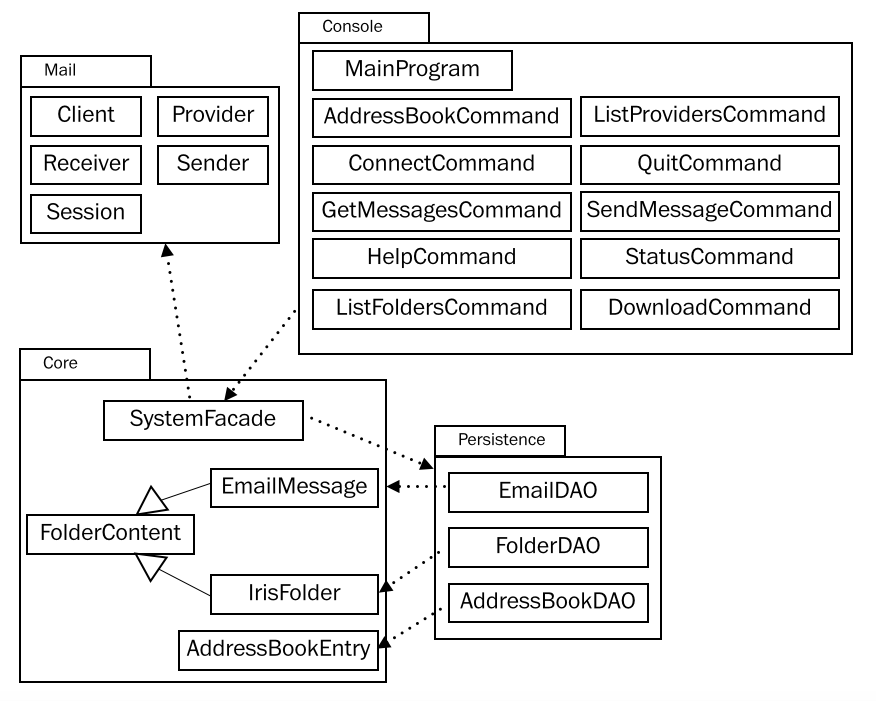
\includegraphics[width=4.5in]{case_study_fig_1.png}
\caption{\texttt{IRIS} Architecture. (UML Notation)}
\label{fig:case_study_fig1}
\end{figure}

The Figure~\ref{fig:case_study_fig1} depicts a simplified view of \texttt{IRIS} architecture. It is decomposed in four packages, namely:

\begin{itemize}
\item{Core: holds the model classes and the fa\c{c}ade.}
\item{Mail: takes care of connecting on providers, send and receiving email messages.}
\item{Persistence: as of base version, implements relational persistence.}
\item{Console: has the entry point of application, and provides commands that allows user to interact with it.}
\end{itemize}

As can be seen on Figure~\ref{fig:case_study_fig1}, the \texttt{SystemFacade} class orchestrates the workflow initiated by the user by issuing a command. Its interactions typically involve calls to \texttt{Mail} and \texttt{Persistence} packages. Note that the \texttt{Console} package are allowed to access only the \texttt{SystemFacade}. The commands classes, by the way, are loaded dinamically by the \texttt{MainProgram}. It searches through the classpath seeking Command interface implementers.

The Multiple Folder feature was implemented in a limited way. Only the \texttt{INBOX} and \texttt{OUTBOX} folders are supported, and are automatically created. By folders, we mean local folders. It must not be confounded with remote folders, that resides on the IMAP server database.

Table~\ref{table:case_study_tab1} shows an overview of the source code metrics of \texttt{IRIS}. All metrics are in good shape, except for Number of Methods by Class and Height of Inheritance Tree, that are outside industry-standard ranges.

\begin{table}[!ht]
%% increase table row spacing, adjust to taste
\renewcommand{\arraystretch}{1.3}
% if using array.sty, it might be a good idea to tweak the value of
% \extrarowheight as needed to properly center the text within the cells
\caption{\texttt{IRIS} metrics}
\label{table:case_study_tab1}
\centering
%% Some packages, such as MDW tools, offer better commands for making tables
%% than the plain LaTeX2e tabular which is used here.
\begin{tabular}{|c|c|c|}
\hline
Metric & Value & Mean Value\\
\hline
LOC & 3035 & 4.87, by method\\
\hline
Methods & 623 & 9.88, by class \\
\hline
Classes & 63 & 3.31, by package \\
\hline
Packages & 19 & \\
\hline
Cyclomatic complexity & 640 & 0.21, by LOC \\
\hline
Fan Out & 453 & 0.59, by call \\
\hline
Calls & 757 & 1.21, by method \\
\hline
Number of Direct Descendants & 0.11 & \\
\hline
Height of inheritance tree & 0.37 & \\
\hline
\end{tabular}
\end{table}

\subsection{First Sprint: extract product line}

\subsection{Second Sprint: Initial evolution of the product line}

% quais features foram introduzidas
% caracterizar o cenario de acordo com o trabalho da Lais Neves em gpce 2011

\subsection{Third Sprint: Final evolution of the product line}


% quais features foram introduzidas
% caracterizar o cenario de acordo com o trabalho da Lais Neves em gpce 2011


\subsection{Metrics and Tools}

% ok, acho que aqui poderiamos discutir nossas metricas de interesse.
% acho que poderiamos focar em acoplamento (ver se Lattix oferece algo),
% estabilidade do codigo, analise de impacto considerando artefatos alterados, artefatos adicionados e
% artefatos removidos. Lembrar que temos interesse em aspectos de configuracao: discussao sobre
% a decomposicao entre Persistencia e AddressBook (acho que com AOP, ficou mais modular, mais facil
% de configurar, etc.)

% descrever tambem as ferramentas e procedimentos usados na medicao. 

\section{Results}

\section{Threats to Validity}

\section{Related Works}

\section{Final Remarks}



\ack This class file was developed by Sunrise Setting Ltd,
Torquay, Devon, UK. Website:\\
\href{http://www.sunrise-setting.co.uk}{\texttt{www.sunrise-setting.co.uk}}

\bibliographystyle{wileyj}
\bibliography{modularity.bib}

\end{document}
